\documentclass[aspectratio=169, 10pt]{beamer}
\usepackage{graphicx} % Required for inserting images
\usepackage{booktabs}
\usepackage{adjustbox}
\usepackage[utf8]{inputenc}
\usepackage{lmodern}
\usepackage{tcolorbox}
\usetheme{Boadilla}
%\usefonttheme{serif}

\usepackage{tikz}
\setbeamertemplate{background}{
  \begin{tikzpicture}[remember picture,overlay]
    \node[anchor=north east, xshift=-5mm, yshift=-3.5mm] at (current page.north east) {
      
\includegraphics[height=.75cm]{pics/WHU_Logo_RGB_Screen.jpg}
    };
  \end{tikzpicture}
}

\usecolortheme[]{dolphin}
\definecolor{WHUblue}{rgb}{.08, .27,.58} % WHU Blue 
\setbeamercolor{structure}{fg=WHUblue}

\setbeamertemplate{itemize item}{\color{WHUblue}$\bullet$}
\setbeamertemplate{itemize subitem}{\color{WHUblue}$\circ$}
\setbeamertemplate{itemize subsubitem}{\color{WHUblue}$\cdot$}

\setbeamertemplate{enumerate items}[default]


\setbeamercolor{block title}{bg=WHUblue!10, fg=WHUblue}
\setbeamercolor{block body}{bg=WHUblue!5, fg=black}
\setbeamertemplate{blocks}[default]  % ohne Schatten

\setbeamercolor{quoteblock title}{fg=WHUblue}
\setbeamercolor{quoteblock body}{bg=WHUblue!5}

\newenvironment{quoteblock}[1]{%
  \begin{beamercolorbox}[colsep*=.75ex, leftskip=1em, rightskip=1em, width=\textwidth, rounded=true]{quoteblock body}
  \textit{#1}
  \end{beamercolorbox}
}{}


\setbeamersize{text margin left=0.75cm, text margin right=0.75cm}

\setbeamertemplate{navigation symbols}{} % Symbole aus

\setbeamertemplate{headline}{%
  \leavevmode%
  \hspace{1em}%
  \usebeamercolor[fg]{section in head/foot}%
  \bfseries\insertsection%
  \vspace{0.5em}%
}

\newcommand{\source}[1]{%
  \tikz[remember picture,overlay]{
    \node[anchor=south east, xshift=-0.5cm, yshift=0.5cm] 
    at (current page.south east) {\scriptsize\color{gray!60}#1};
  }%
}

\setlength{\columnsep}{1pt}

\newcommand{\twocolslide}[5]{%
  \begin{frame}
    \frametitle{#1}
    \begin{columns}[T,onlytextwidth]
      \begin{column}{#4\textwidth} % Left column width
         \vfill
        \begin{minipage}[c][0.9\textheight][c]{\linewidth}
          #2
        \end{minipage}
        \vfill        
      \end{column}
      \begin{column}{#5\textwidth} % Right column width
       \vfill
        \begin{minipage}[c][0.9\textheight][c]{\linewidth}
          #3
        \end{minipage}
        \vfill
      \end{column}
    \end{columns}
  \end{frame}
}

\AtBeginSection[]{
  \begin{frame}[plain]
    \centering
    {\color{WHUblue}\LARGE\bfseries\insertsection}
  \end{frame}
}

\AtBeginSubsection[]{
  \begin{frame}[plain]
    \centering
    \vfill
    {\color{WHUblue}\large\insertsection}
    
    \vspace{1em}
    \color{WHUblue}\Huge\bfseries\insertsubsection
    \vfill
  \end{frame}
}

\title{Business Ethics}
\subtitle{Bachelor of Business Administration WHU}
\author[Rilke]{Prof. Rainer Michael Rilke }
\date{2025}
\begin{document}

\section{Ethical Theories}

%\begin{frame}
%\frametitle{A CEO's Perspective on Business Ethics Education}

%\begin{tcolorbox}[colback=WHUblue!5!white, colframe=WHUblue, title=Quote, fonttitle=\bfseries, sharp corners=south]
%"As you will recall, this CEO described a freshly minted MBA’s answer to his question about what he had learned in his business ethics course: 
%\textbf{“Well, first we learned about all the models of ethical reasoning—you know, utilitarianism, deontology, and so on—and then we learned that whenever you confront an ethical dilemma, you first decide what you want to do and then you select the model of ethical reasoning that will best support your choice.”}
%\end{tcolorbox}
%\source{Source: Mary C. Gentile - Giving Voice to Values (2010)}
%\end{frame}

\subsection{Utilitarianism}



\begin{frame}
\frametitle{Learning Objectives}
 By the end of this lecture, students should be able to:
\begin{itemize}
\item Understand the core principles of consequentialism.
\item Distinguish between different forms (e.g., act vs. rule consequentialism).
\item Evaluate consequentialist reasoning in business contexts.
\item Critically assess strengths and objections to consequentialism.
\item Apply consequentialist ethics to concrete managerial decisions.
\end{itemize}
\end{frame}

\begin{frame}
\frametitle{Opening Activity: Emmely and the Bottle Deposit}

\begin{tcolorbox}[colback=WHUblue!5!white, colframe=WHUblue, title=Scenario, fonttitle=\bfseries, sharp corners=south]
A long-serving supermarket cashier is dismissed without notice after allegedly redeeming two bottle deposit receipts worth €1.30 that did not belong to her.
\end{tcolorbox}

\vspace{1em}

\textbf{Discussion Instructions:}
\begin{itemize}
    \item \textbf{Turn to your neighbor} and discuss: \textit{Was this the right thing to do?}
    \item \textbf{Explain your reasoning} to each other.
    \item \textbf{Take notes:} Each pair should record the reasons discussed.
    \item After 5 minutes, I will call upon some of you to share your reasoning with the class.
\end{itemize}
\end{frame}

\begin{frame}{What is Consequentialism?}

\begin{tcolorbox}[colback=WHUblue!5!white, colframe=WHUblue, title=Definition, fonttitle=\bfseries, sharp corners=south]
Consequentialism is the ethical theory that judges the rightness or wrongness of actions \textbf{solely by their consequences}.
\end{tcolorbox}

\vspace{1em}

\textbf{Key Features:}
\begin{itemize}
    \item \textbf{Teleological structure:} Right acts promote the best overall state of affairs.
    \item \textbf{Impartiality:} Everyone's well-being counts equally.
    \item \textbf{Agent-neutrality:} The identity of the agent does not affect moral assessment.
\end{itemize}

\source{Stanford Encyclopedia of Philosophy (2023)}
\end{frame}

\twocolslide{Utilitarianism: The Classic Form of Consequentialism}{
  \begin{itemize}
    \item \textbf{Jeremy Bentham (1748–1832)}
      \item[] \textit{“Nature has placed mankind under the governance of two sovereign masters, \textbf{pain} and \textbf{pleasure}. It is for them alone to point out what we \textbf{ought to do}, as well as to determine what we \textbf{shall do}.”} \\
  \end{itemize}
  \source{An Introduction to the Principles of Morals and Legislation (1789)}
  
}{  \centering
    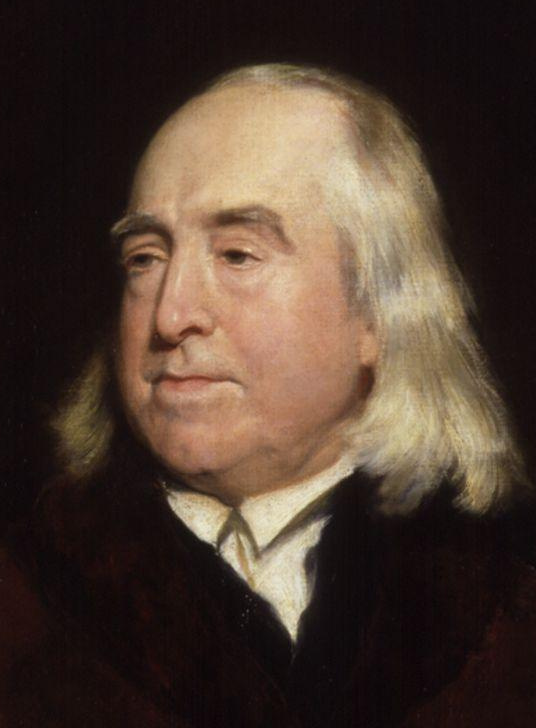
\includegraphics[width=0.5\linewidth]{pics/bentham.jpg} % Replace with actual image file if used
  }{0.6}{0.39}


\begin{frame}{Bentham’s Utilitarianism: Four Core Principles (1)}
    \textbf{Consequences}
    \begin{itemize}
        \item The moral status of an action depends \textbf{only on the value of its consequences}.
        \item Consequentialism adopts a \textbf{teleological structure}: right actions promote the best possible outcomes.
        \item What matters morally is the \textbf{state of affairs} resulting from the action—not the motive, rule, or character.
        \item Two key variants exist:
            \begin{itemize}
                \item \textbf{Actual-consequence consequentialism}: actions are right if they actually produce the best outcomes.
                \item \textbf{Expected-value consequentialism}: actions are right if they are expected to produce the best outcomes, given what the agent knows.
            \end{itemize}
    \end{itemize}
    \source{Bentham, An Introduction to the Principles of Morals and Legislation (1789); SEP (2023)}
\end{frame}

\begin{frame}{Bentham’s Utilitarianism: Four Core Principles (2)}
    \textbf{Utility}
    \begin{itemize}
        \item Utility refers to the overall \textbf{well-being} or \textbf{welfare} of individuals affected by an action.
        \item An action is right if it produces the \textbf{greatest total welfare} across all individuals.
        \item This assumes a \textbf{welfarist value theory}: only individual welfare determines moral value.
        \item Different theories define welfare differently:
            \begin{itemize}
                \item \textbf{Hedonism}: welfare = pleasure minus pain.
                \item \textbf{Desire satisfaction}: welfare = getting what one wants.
                \item \textbf{Objective list}: welfare = achieving valuable life goods (e.g., knowledge, relationships).
            \end{itemize}
        %\item Summarized as: \textit{“The greatest happiness of the greatest number.”}
    \end{itemize}
    \source{Bentham, An Introduction to the Principles of Morals and Legislation (1789); SEP (2023)}
\end{frame}

\begin{frame}{Bentham’s Utilitarianism: Four Core Principles (3)}

\textbf{Hedonism}
\begin{itemize}
    \item A theory of welfare that identifies \textbf{pleasure as the only intrinsic good} and \textbf{pain as the only intrinsic bad}.
    \item Classical utilitarianism adopts \textbf{hedonistic welfarism}: right actions are those that maximize net pleasure.
    \item Morality becomes a matter of producing the \textbf{greatest balance of pleasure over pain}.
    \item Bentham proposed the “\textbf{hedonic calculus}”: a method to measure and compare pleasures and pains based on factors like intensity, duration, certainty, and proximity.
    %\item Criticism: not all pleasures are equal—Mill later distinguished between “higher” and “lower” pleasures.
\end{itemize}

\source{Bentham, \textit{An Introduction to the Principles of Morals and Legislation} (1789); SEP (2023)}
\end{frame}


\begin{frame}{Bentham’s Utilitarianism: Four Core Principles (4)}

\textbf{Impartiality / Agent-Neutrality}
\begin{itemize}
    \item Consequentialist ethics requires \textbf{equal consideration of all individuals' welfare}—no one's well-being counts more than another's.
    \item The theory is \textbf{agent-neutral}: the identity of the agent or their personal relationships do not affect moral evaluation.
    \item Each person’s utility contributes \textbf{equally} to the overall good—this reflects the \textbf{egalitarian foundation} of classical utilitarianism.
    \item This principle supports the idea that morality should be \textbf{generalizable and universally applicable}, not tailored to personal interests.
    %\item Criticism: May conflict with special obligations to family, employees, or communities.
\end{itemize}

\source{Bentham, \textit{An Introduction to the Principles of Morals and Legislation} (1789); SEP (2023)}
\end{frame}


\begin{frame}{Hedonic Calculus: 7 Criteria for Measuring Pleasure}

Quantify the moral value of actions based on the pleasure (or pain) they produce. To make ethics objective and measurable, he proposed that we should assess how much pleasure (or pain) an action produces using seven distinct dimensions. \\

\vspace{1em}

\textbf{The Seven Criteria:}
\begin{enumerate}
    \item \textbf{Intensity} – How strong is the pleasure or pain? \\
   % \small A deep, ecstatic joy is better than mild contentment.
    
    \item \textbf{Duration} – How long does it last? \\
    %\small A week of happiness outweighs a momentary thrill.
    
    \item \textbf{Certainty (or Uncertainty)} – How likely is it to occur? \\
    %\small A 90\% chance of pleasure has more moral weight than a 10\% chance.
    
    \item \textbf{Propinquity (Remoteness)} – How soon will it come? \\
    %\small Immediate pleasures are favored over delayed ones.
    
    \item \textbf{Fecundity} – Will it lead to other pleasures or pains? \\
    %\small The pleasure of exercise may lead to future well-being; cheating may cause guilt.
    
    \item \textbf{Purity} – Is it mixed with pain? \\
    %\small Pure pleasures (e.g. laughter) are better than pleasures mixed with pain (e.g. revenge).
    
    \item \textbf{Extent} – How many people are affected? \\
    %\small A pleasure shared by many is morally better than one felt by a few.
\end{enumerate}

\source{Source: Bentham, \textit{An Introduction to the Principles of Morals and Legislation} (1789)}
\end{frame}

\begin{frame}{Applying the Hedonic Calculus: Triage and Duration}

\textbf{Scenario:}  
During the COVID-19 crisis, a hospital has only one ventilator. Two patients need it:
\begin{itemize}
    \item Patient A: 70-year-old medical doctor
    \item Patient B: 20-year-old business student
\end{itemize}

\vspace{.5em}

\textbf{Bentham’s Duration Criterion:}  
\begin{itemize}
    \item Duration asks: \textit{How long will the resulting pleasure (or well-being) last?}
    \item Saving the 20-year-old may lead to a \textbf{longer expected lifespan}, i.e., more years of utility.
    \item Could be used to justify choosing Patient B to \textbf{maximize total future well-being}.
\end{itemize}

\vspace{.5em}

\begin{tcolorbox}[colback=WHUblue!5!white, colframe=WHUblue, title=Homework, fonttitle=\bfseries, sharp corners=south]
Apply the remaining six criteria of Bentham’s hedonic calculus (Intensity, Certainty, Propinquity, Fecundity, Purity, and Extent) to the triage scenario above. For each criterion, briefly explain how it might influence the ethical decision between Patient A and Patient B.
\end{tcolorbox}


%\textbf{Ethical Tension:}
%\begin{itemize}
%    \item Critics argue this reasoning may be \textbf{ageist} or violate the principle of \textbf{equal human dignity}.
%    \item Highlights a key ethical conflict between \textbf{consequentialist logic} and \textbf{deontological fairness}.
%\end{itemize}

\end{frame}


\begin{frame}{Criticism of COVID Triage Decisions}

\begin{enumerate}
    \item \textbf{Unequal Moral Worth} \\
    Reducing life-and-death decisions to expected utility calculations can imply that some lives are worth less — undermining the principle of equal respect for all persons.

    \vspace{0.5em}
    \item \textbf{Loss of Public Trust} \\
    A system that visibly favors certain groups (e.g., the young) may erode public confidence in healthcare institutions and discourage vulnerable populations from seeking care.

    \vspace{0.5em}
    \item \textbf{Unstable and Arbitrary Judgments} \\
    Case-by-case maximization based on uncertain forecasts (life expectancy, quality of life) invites inconsistency, bias, and moral distress among frontline decision-makers.
\end{enumerate}

\vspace{1em}
\textit{Should we rely on individual outcomes alone, or consider broader principles that guide decisions across cases?}

\end{frame}


\twocolslide{Rule Utilitarianism: A Defense of Act Utilitarianism?}{
      \begin{itemize}
      \item \textbf{John Stuart Mill (1806–1873)}
      \item[] \textit{“It is better to be a human being dissatisfied than a pig satisfied; better to be Socrates dissatisfied than a fool satisfied. And if the fool, or the pig, is of a different opinion, it is only because they know their own side of the question.”} \\
      \end{itemize}  
      \source{Utilitarianism (1863)}
}{ \centering
    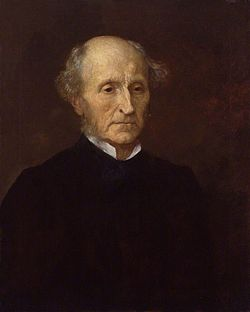
\includegraphics[width=0.5\linewidth]{pics/mill.jpg} % Replace with actual image file if used
  }{0.6}{0.39}

  
\begin{frame}{Dissecting Mill’s Quote}

\textit{“It is better to be} \textcolor{blue}{\textbf{a human being dissatisfied}} \textit{than} \textcolor{blue}{\textbf{a pig satisfied}}%
\textit{; better to be} \textcolor{teal}{\textbf{Socrates dissatisfied}} \textit{than} \textcolor{teal}{\textbf{a fool satisfied}}%
\textit{. And if the fool, or the pig, is of a different opinion, it is only because they} \textcolor{orange}{\textbf{know their own side of the question.”}}

\vspace{.25em}

\uncover<2->{
\tcbset{colback=blue!5,colframe=blue!40!black,boxrule=0.5pt}
\begin{tcolorbox}
Higher (intellectual) pleasures are more valuable than lower (bodily) ones.
\end{tcolorbox}
}

\vspace{0.25em}

\uncover<3->{
\tcbset{colback=teal!5,colframe=teal!60!black,boxrule=0.5pt}
\begin{tcolorbox}
A wise, thoughtful life is better than ignorant contentment.
\end{tcolorbox}
}

\vspace{0.25em}

\uncover<4->{
\tcbset{colback=orange!5,colframe=orange!60!black,boxrule=0.5pt}
\begin{tcolorbox}
Only those who know both pleasures can judge which is better.
\end{tcolorbox}
}
\vspace{0.5em}
\uncover<5->{
Mill introduces a qualitative hierarchy of pleasures. This opens the way for moral rules that promote deeper forms of well-being — not just momentary satisfaction.
}

\end{frame}


\begin{frame}{From Mill’s Higher Pleasures to Rule Utilitarianism (1)}

\textbf{Mill’s Insight:}
\begin{itemize}
    \item Some pleasures (e.g., intellectual, moral, aesthetic) are \textbf{intrinsically higher in quality} than others (e.g., sensual, immediate).
    \item Their value is not just greater in quantity, but in kind — even if they come with dissatisfaction.
    \item Those who have experienced both (e.g., Socrates and the fool) will prefer the higher — suggesting a deeper basis for moral judgment.
\end{itemize}

\vspace{1em}

\textbf{Problem for Act Utilitarianism:}
\begin{itemize}
    \item It evaluates each action only by its total net pleasure — \textbf{regardless of type}.
    \item This risks favoring lower pleasures if they are more immediate or intense.
    %\item It lacks the conceptual space to treat some pleasures as categorically more valuable.
\end{itemize}

\end{frame}

\begin{frame}{From Mill’s Higher Pleasures to Rule Utilitarianism (2)}

\textbf{How This Leads to Rule Utilitarianism:}
\begin{itemize}
    \item Mill’s position implies the need for \textbf{stable moral rules} that promote deeper forms of well-being.
    \item Rule consequentialism evaluates the \textbf{rightness of actions relative to rules}, not individual acts.
    %\item From SEP: “Rule consequentialists evaluate rules in terms of their consequences, and then derive the rightness of acts from the rightness of rules.”
    \item This allows the promotion of higher pleasures — not through immediate outcomes, but by guiding behavior through \textbf{socially beneficial norms}.
\end{itemize}

\vspace{1em}
\textbf{Conclusion:}  
Mill’s elevation of higher pleasures demands a system of values and behaviors that cannot be justified act-by-act — but only through general principles that structure moral life.

\source{Stanford Encyclopedia of Philosophy (2023), “Consequentialism”, § What is Right Relative to Rules}
\end{frame}


\begin{frame}{Example: TikTok vs. Reading}

\textbf{Scenario:} Should a student spend free time on TikTok or reading?

\vspace{0.5em}
\textbf{Act Utilitarianism:}
\begin{itemize}
    \item TikTok gives quick, easy pleasure.
    \item If it brings more immediate enjoyment, it’s the “right” choice.
    \item Ignores long-term or qualitative value.
\end{itemize}

\vspace{0.5em}
\textbf{Mill’s View (Higher Pleasures):}
\begin{itemize}
    \item Reading develops intellect and character—\textbf{higher} pleasures.
    \item Those who know both prefer reading’s deeper value.
\end{itemize}

\vspace{0.5em}
\textbf{Rule Utilitarianism:}
\begin{itemize}
    \item Societies should promote habits (like reading) that foster higher well-being.
    \item This requires \textbf{rules}, not just case-by-case pleasure.
\end{itemize}

\end{frame}

\begin{frame}{Mill: Rules and Utility}

\textbf{Rule Utilitarian Principle:} \\
An act \(A\) in circumstance \(C\) is right if, were everyone to follow the rule “If in \(C\), do \(A\),” total utility would be at least as great as for any alternative rule.

\vspace{0.5em}
\textbf{Example: Promise-keeping}
\begin{itemize}
    \item Situation: You have made a promise (\(C\)).
    \item Options: \(A_1\) = keep it; \(A_2\) = break it (assume \(A_2\) yields more utility in this case).
    \item  Rules: \(R_1\) = “If you made a promise, keep it.” \\
    \phantom{Rules: } \(R_2\) = “If you made a promise, break it.”
\end{itemize}

%\vspace{0.5em}
%\textbf{Conclusion:} \\
%If everyone followed \(R_1\), total utility would be higher than if everyone followed \(R_2\). \\
%\textit{→ So, keep your promise, even if breaking it seems better in this case.}

\end{frame}

\begin{frame}{Why Keeping Promises (Rule \( R1 \)) Maximizes Utility}

\textbf{Why would society-wide adoption of \( R1 \) produce more utility than \( R2 \)?}

\begin{itemize}
    \item \textbf{Trust and cooperation}: Keeping promises builds reliable expectations and enables long-term relationships — essential for families, business, and public life.
    
    \item \textbf{Social stability}: Rule \( R1 \) supports contracts, institutions, and planning. Rule \( R2 \) would erode social order and make commitments meaningless.

    \item \textbf{Moral integrity}: Acting on \( R1 \) supports a sense of responsibility and self-respect; breaking promises weakens ethical standards and relationships.

    \item \textbf{Lower social cost}: With \( R1 \), people don't need to constantly monitor or enforce agreements — saving resources and emotional energy.
\end{itemize}

\vspace{0.5em}
\textit{Conclusion: Even if breaking a promise brings short-term benefits, following a rule to keep promises promotes the greatest good in the long run.}

\end{frame}


\begin{frame}{Emmely and the Bottle Deposit: Conclusion}

\begin{tcolorbox}[colback=WHUblue!5!white, colframe=WHUblue, title=Legal Outcome, fonttitle=\bfseries, sharp corners=south]
    In 2010, the German Federal Labour Court ruled the dismissal invalid, emphasizing the principle of proportionality in light of the minor offense and her long service record.
\end{tcolorbox}

\vspace{0.5em}
\textbf{Ethical Relevance:} \\
\begin{itemize}
  \item    From a \textbf{consequentialist} view, dismissal could be justified to deter theft or preserve trust.
  \item  Critics argue the negative impact on Emmely outweighs minimal benefit to the firm.
  \item  A \textbf{rule-consequentialist} might reject such dismissals as leading to injustice and demoralization.
  \item  Highlights the limits of outcome-based ethics in evaluating fairness, dignity, and proportionality.
\end{itemize}

\end{frame}


\end{document}